\chapter{Literature Review}

This section will discuss the background literature relating to this project.

\section{Machine Learning}

\begin{justify}
Classification is the process of mapping observations into predefined classes, based on a set of training data. Some classification algorithms include Decision Tree, Support Vector Machine (SVM), Naïve Bayes, Random Forest, K-means, Logistic Regression and Nearest Neighbour.

There are two main approaches to text classification using machine learning; supervised and unsupervised learning. Supervised learning involves labelled data. There are input variables (x) and output variables (y) and an algorithm is used to train the mapping function from the input to the output (y = f(x)). This mapping function that has been trained is then applied to new unseen data. Unsupervised learning, uses unlabelled data and only has input variables (x) with no output variables. An algorithm is used to find patterns directly from the data. It is generally not used for classification but to discover unknown patterns in data. A supervised machine learning approach will be taken in this research.
\end{justify}

\section{Sentiment Analysis}

Lexicon based..

Machine Learning..

\section{Recommender Systems}

A recommender system is...

\section{Twitter Analysis}

In this section, research that has been carried out on Twitter data will be discussed.

All standard learning algorithms must be adapted to the domain on which they will be used in order to achieve optimum performance. The classifier applied to Twitter data is no exception. It must be fine tuned to get the best accuracy. Tweets are very different to normal longer form text and need to be treated differently. Tweets are very informal, using casual language and slang. They contain things like hashtags, emoticons, twitter handles, URLs, images, videos and gifs.

\section{Preprocessing}

A Support Vector Machine (SVM) is a discriminative classifier, first introduced by Cortes and Vapnik \cite{Vapnik1995,Vapnik21995}. It finds the optimum hyperplane that separates the data into classes. The aim of a SVM is to maximise the margin (distance) between the hyperplane and the support vectors (data points closest to the hyperplane). SVMs have been used successfully for text classification \textcolor{red}{EXAMPLES}.

Naïve Bayes (NB) is a popular supervised learning method for text classification. It is a probabilistic classifier, calculating the probability that an observation belongs to a particular class. NB is based on applying Bayes Rule along with the ‘naïve’ assumption that features are conditionally independent. In the case of text classification, this assumes all words are independent, which is untrue. Bayes Rule is as follows:  \[P(A\mid B)=\frac{P(B\mid A)\:P(A)}{P(B)}\] 

A. Bermingham and A. F. Smeaton \cite{Berm2010} investigate the performance of both Support Vector Machines (SVM) and Multinomial Naïve Bayes (MNB) in classifying the sentiment of short versus long form documents. The short form documents used were microblogs from Twitter and micro-reviews from Blippr. The long form documents were TREC Blog06 Corpus and Pang and Lees Movie Review Corpus \cite{panglee2004}. A maximum accuracy of 74.85\% was achieved with MNB versus 73.45\% with SVM. Overall MNB achieves better accuracy than SVM on the short form documents, suggesting that MNB may be useful for the classification of tweets as reviews.

Another point of interest is the kind of feature extraction that performed well for the long versus short form documents. Extending the unigram feature representation improved classification accuracy for the long form documents, but did not for the short form documents. However POS (part-of-speech) features and punctuation aided classification of the short form documents. 

Logistic Regression (LR) is a linear classifier. LR uses the logistic function, known also as the sigmoid function or logit function to model the data. This is an S-shaped curve, taking real valued inputs and mapping them to the range 0 – 1. The logistic function is as follows: \[g(z)=1/(1+e^{-z})\]
LR models the probability that an observation belongs to a particular class. The coefficients of the LR algorithm are estimated from the training data, using maximum likelihood estimation or gradient descent.

\textcolor{red}{LR for text classfication}

An Ensemble Classifier aggregates various individual base classifiers. It has been demonstrated that an ensemble classifier generally performs better than individual classifiers \cite{Opitz1999}. Ankit and N. Saleena \cite{Ankit2018} propose an ensemble classifier for the sentiment analysis of tweets. The base classifiers include Naive Bayes, Random Forest, Support Vector Machine and Logistic Regression. The ensemble classifier outperforms each of the individual base classifiers.
\textcolor{red}{Two possible ensemble techniques are boosting and bagging.}

Ensemble classifiers, combines the effect of multiple learning algorithms to achieve better performance than the individual learning algorithms. There are averaging ensemble methods and boosting ensemble methods. Averaging methods include Bagging and Forests of randomized trees. They average the base estimators. Boosting methods include Ada Boost and Gradient Tree Boosting. They give an ensemble output which is the sequential effect of base classifiers. 

M. Kanakaraj and R. M. R. Guddeti \cite{Kanakaraj2015} compared several classifiers and ensemble methods on how well they performed classifying the sentiment of tweets as positive, negative or neutral. The classifiers were Support Vector Machine, Baseline, Maximum Entropy and Naive Bayes. The ensemble classifier performed the best. The ensemble method that performed the best was extremely randomized trees. Their system consisted of a data gathering module, a data processing module, a training and classification module and classification output. Data was gathered using the Twitter API. The data processing module removed any repeated letters and words, applied word sense tagging, removed any hash tags, URLs or names, applied part-of-speech (POS) tagging, applied stemming synonyms from WordNet and finally formed feature vectors. The training and classification module applied SVM, Baseline, MaxEnt, Naive Bayes and each of the ensemble methods, extremely randomized trees, random forest, adaboost, and decision tree.

A. Go, R. Bhayani, and L. Huang \cite{Go2009} proposed the  idea of creating a training set of tweets, labelled as positive or negative based on the emoticons they contain. The dataset produced (Stanford Sentiment 140) was used to train Naive Bayes, Maximum Entropy, and Support Vector Machine classifiers. They report the best accuracy (83\%) with the Maximum Entropy Classifier. Their work helped address the problem of creating large labelled datasets to train classifiers. This can be a very time-consuming, costly and labour-intensive process. The dataset produced has been used in many other studies, including the above mentioned Ensemble Classifier study \cite{Ankit2018}.

\textcolor{red}{How does the Max Ent work?}

A. Rane and A. Kumar compare seven different classifiers (Decision Tree, Random Forest, SVM, K-Nearest Neighbours, Logistic Regression, Gaussian Naïve Bayes and AdaBoost) for the sentiment analysis of Twitter Data about US Airline Services \cite{Rane2018}. 
\begin{wrapfigure}{r}{0.5\textwidth}
    \centering
    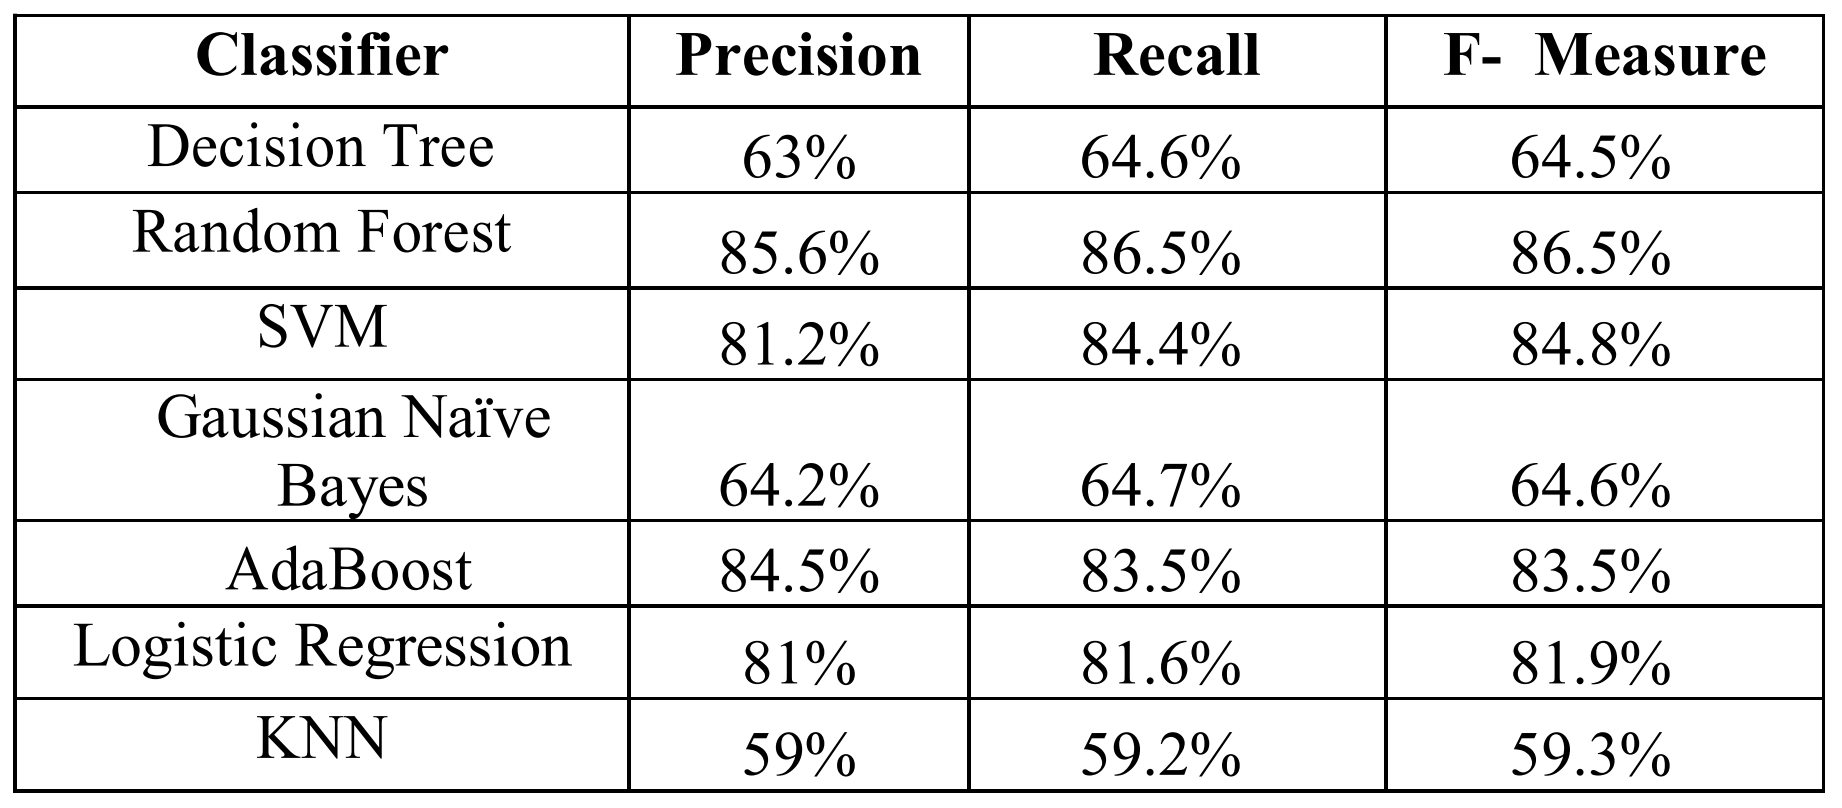
\includegraphics[width=0.5\textwidth]{literature_review/arane_classifier_results.PNG}
    \caption{Accuracy of Classifier Results from the study by A. Rane and A. Kumar \cite{Rane2018}}
\end{wrapfigure}
The Random Forest Classifier performed the best, with reported precision of 85.6\%. The research makes use of doc2vec.

\textcolor{red}{How does Random Forest work?}

\textcolor{red}{Feature Representation: DOC2VEC}

M. Rathi, A. Malik, D. Varshney, R. Sharma, and S. Mendiratta \cite{Raithi2018} tested SVM, Adaboosted Decision Tree and Decision Tree Classifiers, for the sentiment analysis of tweets. TFIDF (term frequency inverse document frequency) Vectorization is applied during pre-processing. Using TFIDF gives a measure of how important a word is within the dataset. A word that is frequent in an individual document but infrequent in the dataset is considered important. The weights from TFIDF are applied to the dataset emphasising the contribution of some words and reducing the contribution of others. They found the Decision Tree Classifier performed best  (accuracy: 84\%) followed by the SVM (accuracy: 82\%) and then the Adaboosted (accuracy: 67\%). 

The Stanford NLP (Natural Language Processing) Group's Sentiment Analyser \cite{stanfordSentiment2013} introduced a Recursive Neural Tensor Network (RNTN) along with a Sentiment Treebank. The Sentiment Treebank extended the corpus of movie reviews originally collected by Pang and Lee \cite{panglee2004}. The sentences in the movie review corpus were relabeled at a phrase level, producing a sentiment labelled parse-tree for each review. The Sentiment Treebank produced had more finely grained sentiment labels than the original corpus. It improved how the compositional effects of sentiment in language were captured. For example a word may be positive in one context but negative in another. In this sentence, 'The phone has a really long battery life', long is positive, however in this sentence, 'The website took so long to load', long is negative.

\begin{wrapfigure}{l}{0.6\textwidth}
    \centering
    \setlength{\fboxsep}{0pt}
    \setlength{\fboxrule}{0.01pt}
    \setlength{\belowcaptionskip}{-20pt}
    \fbox{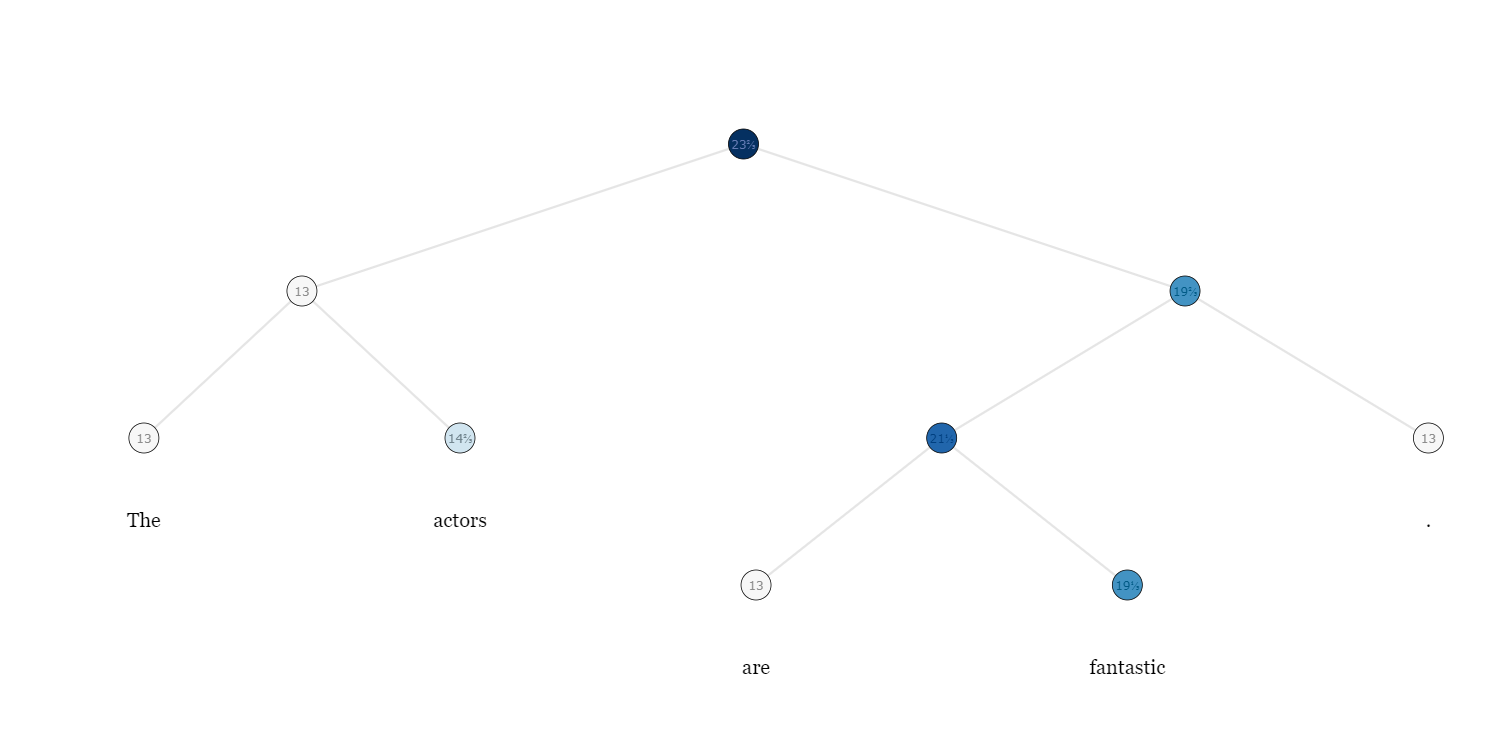
\includegraphics[width=0.6\textwidth]
    {literature_review/sample_treebank.PNG}}
    \caption{A labelled movie review in the Stanford NLP Sentiment Treebank \cite{stanfordSentiment2013}}
\end{wrapfigure}

All classification models trained with the new dataset saw a significant increase in accuracy. These included Naive Bayes, Support Vector Machines, and other recursive neural networks. The RNTN achieved the highest accuracy of 85.4\% in single sentence positive/negative classification.

S. Bhuta, A. Doshi, U. Doshi, and M. Narvekar \cite{Bhuta2014} reviewed different methods for the sentiment analysis for text, with a focus on Twitter. A lexicon based approach works by classifying a sentence based on the number of opinion words (positive or negative words) in the sentence. A sentiment score is calculated based on the ratio of positive to negative words. Unlike supervised machine learning methods no training data is required. However, a lexicon is required and these are not available for every language. The lexicon approach has limitations, it does not allow for a term to be positive in one context but negative in another. It also cannot deal with an opinion being expressed towards multiple entities in a single sentence.

Three supervised learning methods were investigated, Naive Bayes, Maximum Entropy and Support Vector Machines. Supervised learning methods generally outperform the lexicon based approach. They are however very dependent on the size and quality of the set of training data. The accuracy of a classifier depends on the features selected and the domain in question. A method that performs well on a set of reviews from Tripadvisor will not perform as well on a set of Tweets. Each method needs to be adapted to the specific domain it will be used on.

Naive Bayes is a simple probabilistic classifier that uses Bayes theorem. There are two first order probabilistic models for Naive Bayes, Bernoulli(shorter vocab sizes) and Multinomial (longer vocab sizes). Bernoulli performs better on smaller vocabularies and Multinomial performs better on larger vocabularies. The bigram NB outperformed the unigram. ${X}^2$ feature selection improved the accuracy.

Maximum Entropy is a probability distribution estimation technique. The principle of Maximum Entropy is that if not much is known about the data the distribution should be as uniform as possible, i.e. have the maximum entropy. The improved iterative scaling algorithm is used to find the solution.An advantage over Naive Bayes is it does not suffer from the independence assumption.ME does suffer from over-fitting, which can be improved using  a maximum a posteriori.

Support Vector Machines find the hyper plane with the maximum margin between the classes. It is useful for Twitter data as it can handle large feature spaces. A disadvantage of SVM is that it is a black box method. It is hard to know what is having an effect on the algorithm and how to improve it.

The system proposed consists of four stages, extraction, pre-processing, analysis and knowledge discovery. Extraction involves capturing real time data from Twitter. In the pre-processing stage non-english tweets are filtered out, features are selected, any Twitter handles are removed, any re-tweet symbols (RT) are removed, and exaggeration is removed (goooood -> good). The analysis stage is where the sentiment analysis is performed using a classifier or lexicon approach. Finally in knowledge discovery the sentiment analysis is related to geographical locations and events, to gauge the opinion of the population on that event.

Takehara, T. and Miki, S. and Nitta, N. and Babaguchi, N. propose a recommender system \cite{takeharaContext2012}, that recommends restaurants to users along with contextual information taken from Twitter. They use a rule based system. Relevant keywords are extracted from reviews from Tabelog (a japanese review site) and used to search Twitter for the contextual information. Nouns are extracted from Tabelog using POS tagging. Those characteristically used for assessing restaurants in each area are selected as keywords, categorized as area related or restaurant related. Finally tweets containing more than two nouns from each set of keywords (area and restaurant) are selected as contextual information.



